
\documentclass[11pt]{exam} % https://www.ctan.org/pkg/exam?lang=en

\usepackage[lmargin=1.in,rmargin=1.in,tmargin=1.in,bmargin=1in]{geometry}
\usepackage{setspace}
\usepackage[pdftex]{graphicx}
\usepackage{titling}
\usepackage[
	pdfauthor={Brian Weinstein},
	pdftitle={Homework 1},
	bookmarks=true,
	colorlinks=true,
	linkcolor=blue,
	urlcolor=blue,
	citecolor=blue,
	pdftex,
	linktocpage=true
	]{hyperref}
\usepackage[textsize=tiny]{todonotes}
\usepackage{float}
\setlength\parindent{0pt}
\usepackage{lipsum}
\usepackage{amsmath}
\usepackage{caption}


\qformat{\textbf{Problem \thequestion: \thequestiontitle}\quad \hfill}


\pagestyle{headandfoot}
\runningheadrule
\firstpageheader{}{}{}
\runningheader{\theauthor}{\thetitle}{\thedate}
\firstpagefooter{}{\thepage}{}
\runningfooter{}{\thepage}{}


\usepackage{xcolor}
\usepackage{adjustbox}
\usepackage{verbatim}
\definecolor{shadecolor}{rgb}{.9, .9, .9}

\newenvironment{code}%
   {\par\noindent\adjustbox{margin=1ex,bgcolor=shadecolor,margin=0ex \medskipamount}\bgroup\minipage\linewidth\verbatim}%
   {\endverbatim\endminipage\egroup}

\newenvironment{codeSmall}%
   {\par\noindent\adjustbox{margin=1ex,bgcolor=shadecolor,margin=0ex \medskipamount}\bgroup\minipage\linewidth\verbatim\footnotesize}%
   {\endverbatim\endminipage\egroup}

\newcommand{\ramsey}{\href{http://www.statisticalsleuth.com/}{Ramsey }}



\begin{document}


\title{STAT W4201 001, Homework 8}
\author{Brian Weinstein (bmw2148)}
\date{Apr 6, 2016}
\maketitle

Code is attached here and also posted at \href{https://github.com/BrianWeinstein/advanced-data-analysis}{https://github.com/BrianWeinstein/advanced-data-analysis}. Where relevant, code snippets and output are are included in-line.

\begin{questions}


\titledquestion{\ramsey 12.17}
\setlength{\parindent}{1em}


\textit{It is desired to determine whether the pollution variables (13, 14, and 15) are associated with mortality, after the other climate and socioeconomic variables are accounted for. (Note: These data have problems with influential observations and with lack of independence due to spatial correlation; these problems are ignored for purposes of this exercise.)}

\begin{parts}
\setlength{\parindent}{1em}


\part \textit{With mortality as the response, use a Cp plot and the BIC to select a good-fitting regression model involving weather and socioeconomic variables as explanatory. To the model with the lowest Cp, add the three pollution variables (transformed to their logarithms) and obtain the p-value from the extra-sum-of-squares F-test due to their addition.}

A matrix of pairwise scatterplots is shown in Figure \ref{fig:1a_pairs}.

\begin{figure}[!h]
	\centering
	\captionsetup{width=0.8\textwidth}
	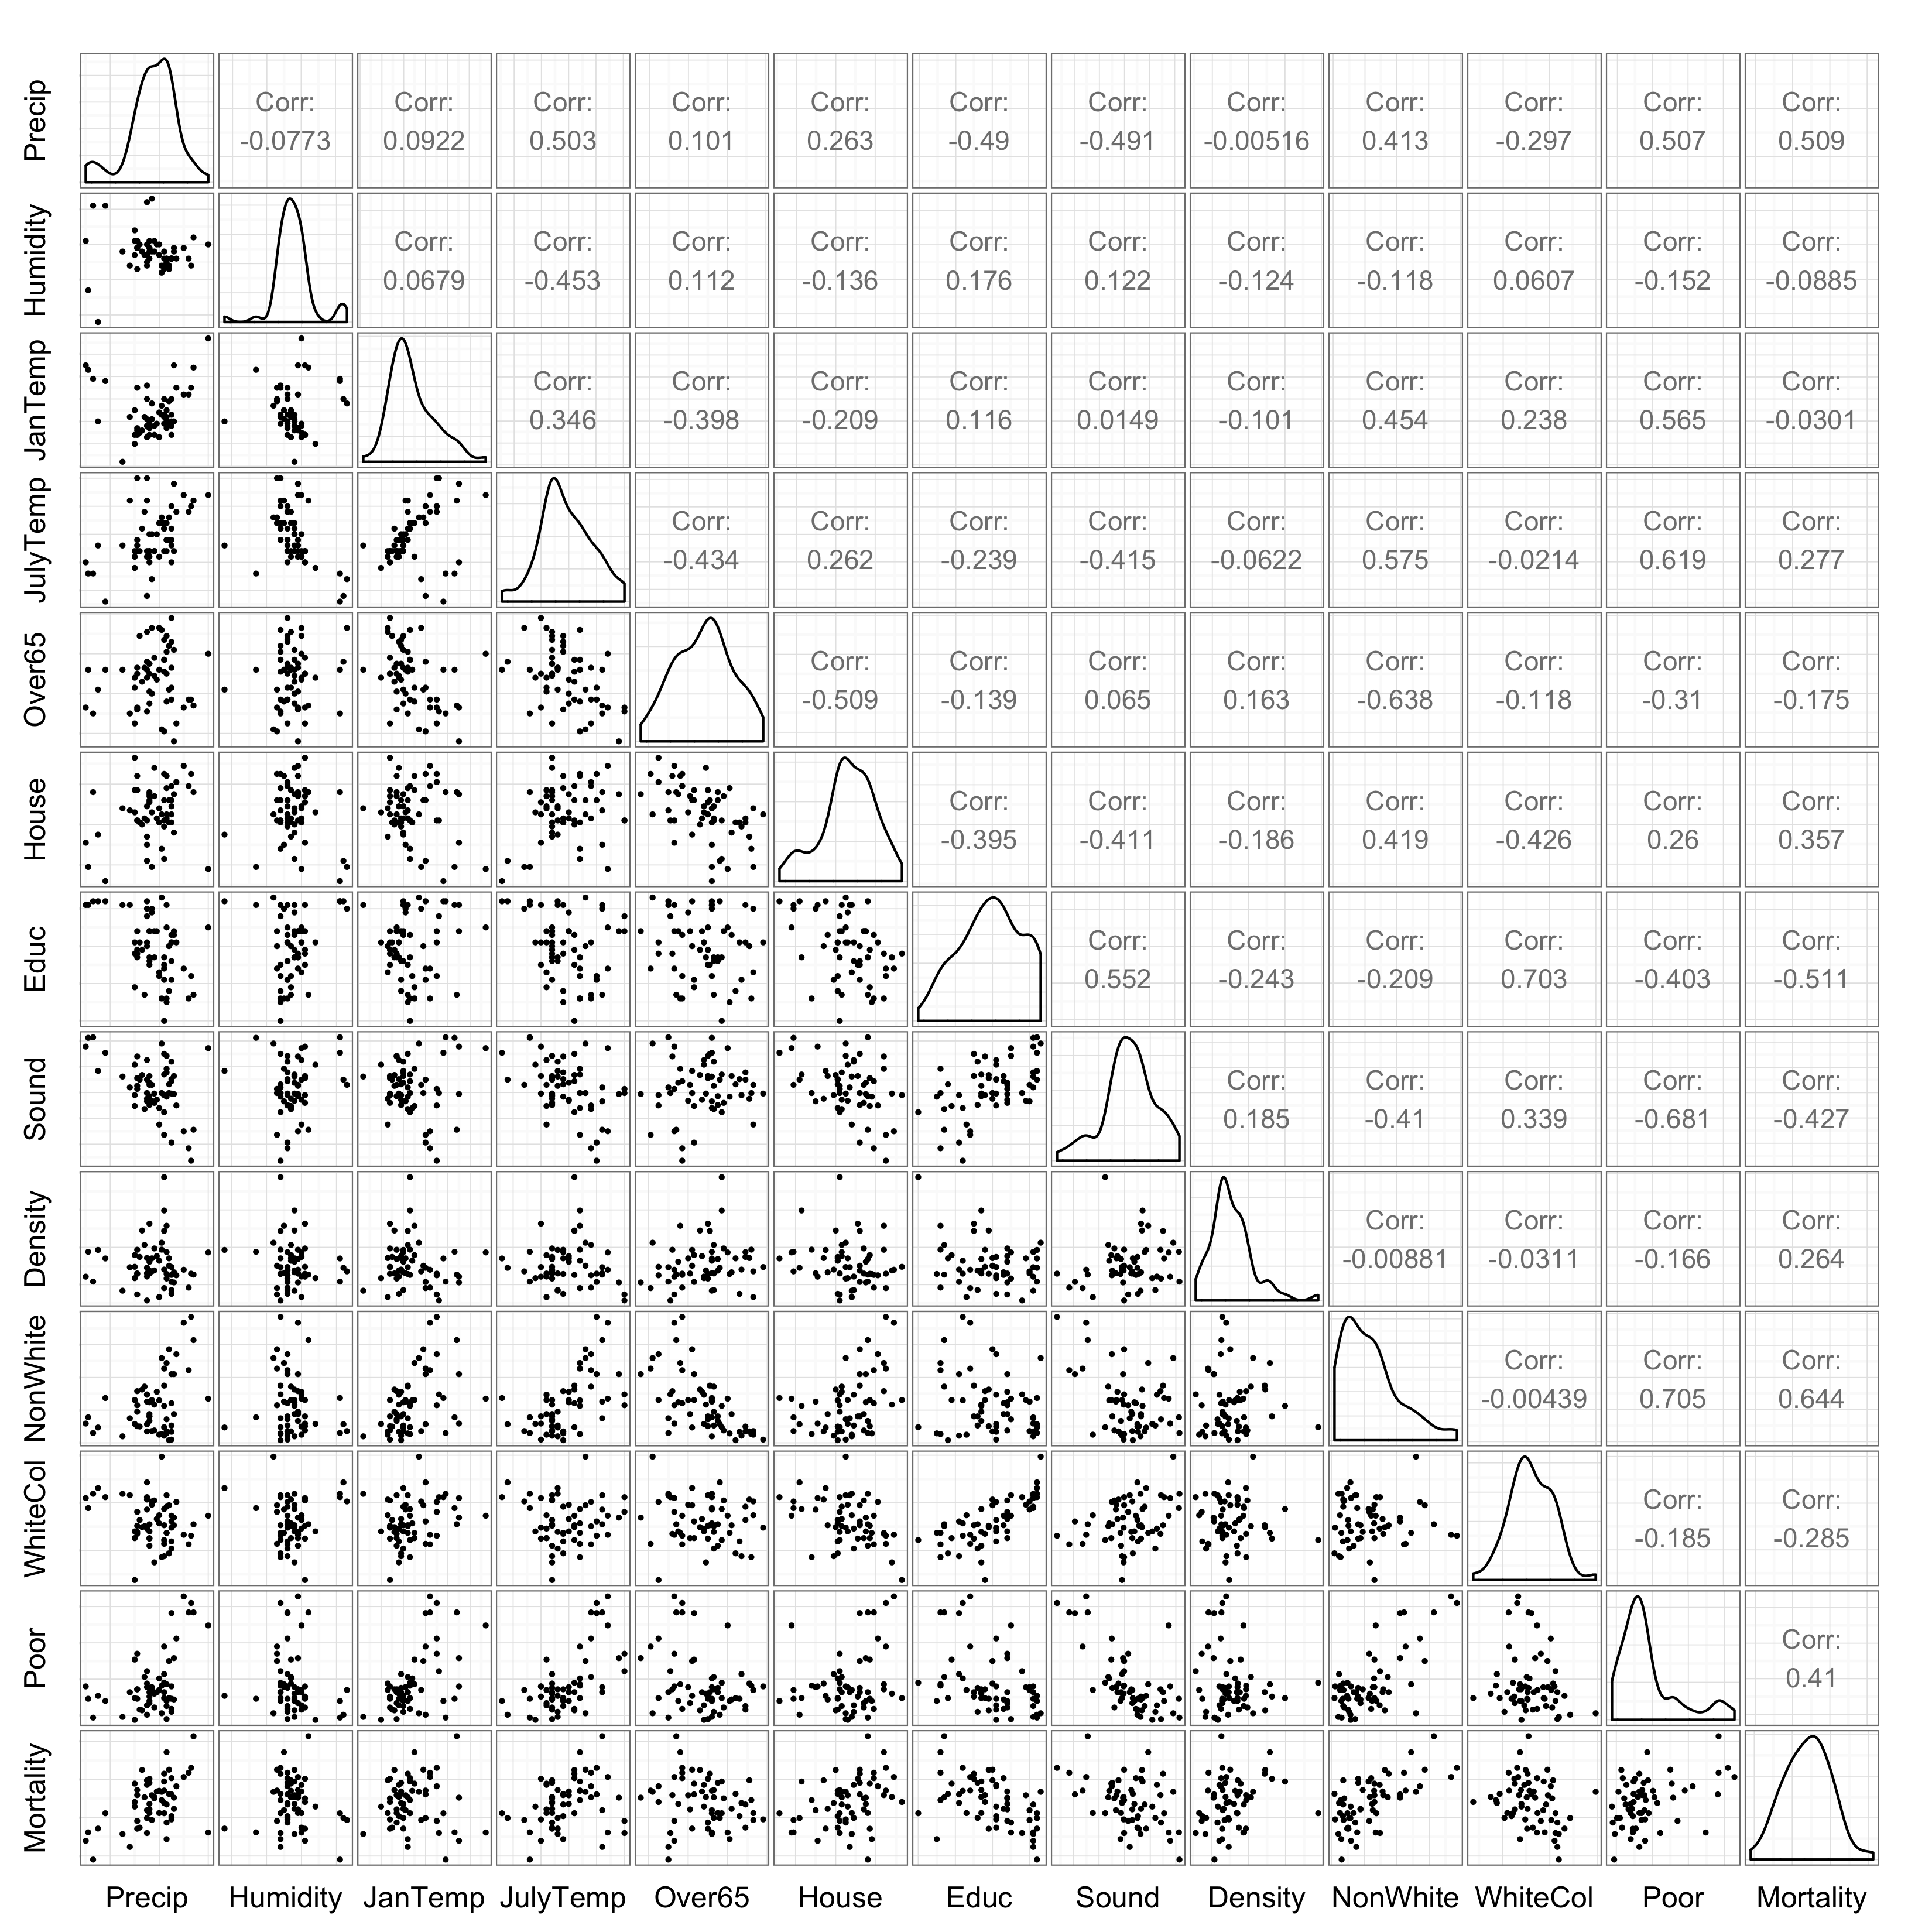
\includegraphics[width=\textwidth]{1a_pairs.png}
	\caption{Pairwise scatterplots of the weather and socioeconomic varibles from the ``Pollution and Mortality'' dataset.}
	\label{fig:1a_pairs}
\end{figure}

Initial investigation of the pairwise scatterplots indicate a couple of things.
\begin{itemize}

\item The effect of the JanTemp, JulyTemp, Over65, and House variables on Mortality are all nonlinear. As each of these variables increases (marginally, at least), Mortality first increases and then decreases. Adding quadratic terms for each of these variables will help model this behavior.

\item Many of the explanatory variables are highly correlated (e.g., JanTemp and JulyTemp, Educ and Sound, Humidity and WhiteCol, etc.). The inclusion of all of these variables will likely be unnecessary in the final model, but we keep them here so that it's unlikely we miss an important relationship during initial investigation.

\end{itemize}

Using the \textit{leaps::regsubsets} R function, we first do an exhaustive search over all $2^16$ possible models (using the original 12 weather and socioeconomic variables, and the 4 squared terms), recording the Cp and BIC for the best few models of each size. We then ignore the models that include a squared variable but don't include the associated linear variable (as per section 12.6).

A Cp plot is shown in Figure \ref{fig:1a_cp} for the remaining models. To reduce clutter, I've only included those models with relatively low Cp statistics.

\begin{figure}[!h]
	\centering
	\captionsetup{width=0.8\textwidth}
	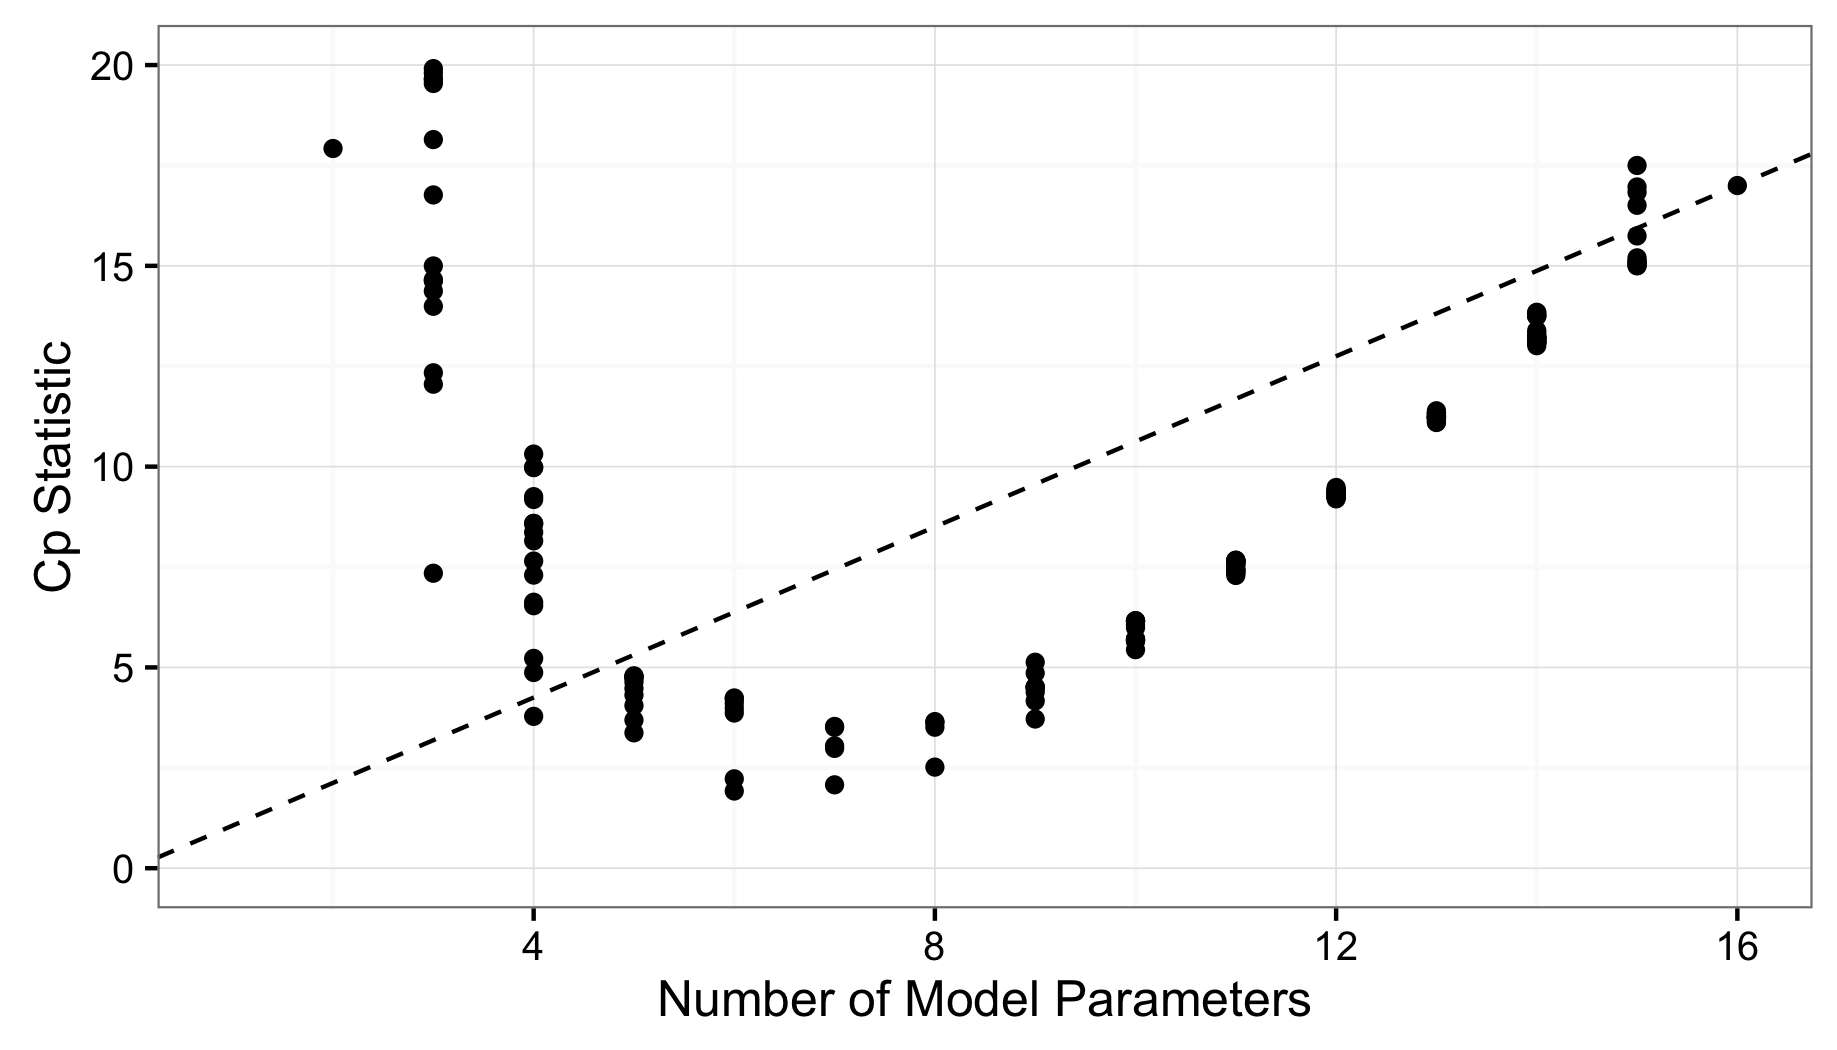
\includegraphics[width=4.25in]{1a_cp.png}
	\caption{Cp plot for the ''good subset models`` with relatively low Cp statistics.}
	\label{fig:1a_cp}
\end{figure}

The model with the lowest Cp statistic is the one that includes Precip, JanTemp, JulyTemp, Educ, Density, and NonWhite, plus an intercept term. For this model, the Cp statistic is $1.922$. This model has the 3rd lowest BIC, and we continue with this set of variables for the remainder of the problem.

To the 6-variable model, we add the log-transformed pollution variables and perform an extra-sum-of-squares F-test as shown below.

\begin{codeSmall}
> anova(lmBestSubsetPoll, lmBestSubset)
Analysis of Variance Table

Model 1: Mortality ~ Precip + JanTemp + JulyTemp + Educ + Density + NonWhite + 
    log(HC) + log(NOX) + log(SO2)
Model 2: Mortality ~ Precip + JanTemp + JulyTemp + Educ + Density + NonWhite
  Res.Df   RSS Df Sum of Sq     F   Pr(>F)   
1     50 52712                               
2     53 66518 -3    -13806 4.365 0.008313 **
---
Signif. codes:  0 ‘***’ 0.001 ‘**’ 0.01 ‘*’ 0.05 ‘.’ 0.1 ‘ ’ 1
\end{codeSmall}

Using the results from the 6-variable model and the 9-variable model (including the 6 variables, plus the 3 pollution variables), the data provides convincing evidence that the three pollution variables are associated with mortality (p-value = 0.008313; extra sum of squares F-test).


\part \textit{Repeat part (a) but use a sequential variable selection technique (forward selection, backward elimination, or stepwise regression). How does the p-value compare?}

Using forward selection, we select a model that includes NonWhite, Educ, JanTemp, House, JulyTemp, Precip, and Density, plus an intercept term.

To this 7-variable model, we add the log-transformed pollution variables and perform an extra-sum-of-squares F-test as shown below.

\begin{codeSmall}
> anova(lmForwardSubsetPoll, lmForwardSubset)
Analysis of Variance Table

Model 1: Mortality ~ NonWhite + Educ + JanTemp + House + JulyTemp + Precip + 
    Density + log(HC) + log(NOX) + log(SO2)
Model 2: Mortality ~ NonWhite + Educ + JanTemp + House + JulyTemp + Precip + 
    Density
  Res.Df   RSS Df Sum of Sq      F   Pr(>F)   
1     49 50403                                
2     52 63955 -3    -13552 4.3915 0.008162 **
---
Signif. codes:  0 ‘***’ 0.001 ‘**’ 0.01 ‘*’ 0.05 ‘.’ 0.1 ‘ ’ 1
\end{codeSmall}

Using the results from the 7-variable model and the 10-variable model (including the 7 variables, plus the 3 pollution variables), the data provides convincing evidence that the three pollution variables are associated with mortality (p-value = 0.008162; extra sum of squares F-test). Using forward selection, the p-value is almost identical to (negligibly smaller than) the one found using the model in part (a).

\end{parts}




\titledquestion{\ramsey 12.20}




\titledquestion{\ramsey 20.11}




\titledquestion{\ramsey 20.15}




\titledquestion{} % Problem 5




\titledquestion{} % Problem 6




\end{questions}

%\listoftodos

\end{document}